% Options for packages loaded elsewhere
% Options for packages loaded elsewhere
\PassOptionsToPackage{unicode}{hyperref}
\PassOptionsToPackage{hyphens}{url}
\PassOptionsToPackage{dvipsnames,svgnames,x11names}{xcolor}
%
\documentclass[
]{article}
\usepackage{xcolor}
\usepackage[margin=1in]{geometry}
\usepackage{amsmath,amssymb}
\setcounter{secnumdepth}{5}
\usepackage{iftex}
\ifPDFTeX
  \usepackage[T1]{fontenc}
  \usepackage[utf8]{inputenc}
  \usepackage{textcomp} % provide euro and other symbols
\else % if luatex or xetex
  \usepackage{unicode-math} % this also loads fontspec
  \defaultfontfeatures{Scale=MatchLowercase}
  \defaultfontfeatures[\rmfamily]{Ligatures=TeX,Scale=1}
\fi
\usepackage{lmodern}
\ifPDFTeX\else
  % xetex/luatex font selection
\fi
% Use upquote if available, for straight quotes in verbatim environments
\IfFileExists{upquote.sty}{\usepackage{upquote}}{}
\IfFileExists{microtype.sty}{% use microtype if available
  \usepackage[]{microtype}
  \UseMicrotypeSet[protrusion]{basicmath} % disable protrusion for tt fonts
}{}
\makeatletter
\@ifundefined{KOMAClassName}{% if non-KOMA class
  \IfFileExists{parskip.sty}{%
    \usepackage{parskip}
  }{% else
    \setlength{\parindent}{0pt}
    \setlength{\parskip}{6pt plus 2pt minus 1pt}}
}{% if KOMA class
  \KOMAoptions{parskip=half}}
\makeatother
% Make \paragraph and \subparagraph free-standing
\makeatletter
\ifx\paragraph\undefined\else
  \let\oldparagraph\paragraph
  \renewcommand{\paragraph}{
    \@ifstar
      \xxxParagraphStar
      \xxxParagraphNoStar
  }
  \newcommand{\xxxParagraphStar}[1]{\oldparagraph*{#1}\mbox{}}
  \newcommand{\xxxParagraphNoStar}[1]{\oldparagraph{#1}\mbox{}}
\fi
\ifx\subparagraph\undefined\else
  \let\oldsubparagraph\subparagraph
  \renewcommand{\subparagraph}{
    \@ifstar
      \xxxSubParagraphStar
      \xxxSubParagraphNoStar
  }
  \newcommand{\xxxSubParagraphStar}[1]{\oldsubparagraph*{#1}\mbox{}}
  \newcommand{\xxxSubParagraphNoStar}[1]{\oldsubparagraph{#1}\mbox{}}
\fi
\makeatother

\usepackage{color}
\usepackage{fancyvrb}
\newcommand{\VerbBar}{|}
\newcommand{\VERB}{\Verb[commandchars=\\\{\}]}
\DefineVerbatimEnvironment{Highlighting}{Verbatim}{commandchars=\\\{\}}
% Add ',fontsize=\small' for more characters per line
\usepackage{framed}
\definecolor{shadecolor}{RGB}{241,243,245}
\newenvironment{Shaded}{\begin{snugshade}}{\end{snugshade}}
\newcommand{\AlertTok}[1]{\textcolor[rgb]{0.68,0.00,0.00}{#1}}
\newcommand{\AnnotationTok}[1]{\textcolor[rgb]{0.37,0.37,0.37}{#1}}
\newcommand{\AttributeTok}[1]{\textcolor[rgb]{0.40,0.45,0.13}{#1}}
\newcommand{\BaseNTok}[1]{\textcolor[rgb]{0.68,0.00,0.00}{#1}}
\newcommand{\BuiltInTok}[1]{\textcolor[rgb]{0.00,0.23,0.31}{#1}}
\newcommand{\CharTok}[1]{\textcolor[rgb]{0.13,0.47,0.30}{#1}}
\newcommand{\CommentTok}[1]{\textcolor[rgb]{0.37,0.37,0.37}{#1}}
\newcommand{\CommentVarTok}[1]{\textcolor[rgb]{0.37,0.37,0.37}{\textit{#1}}}
\newcommand{\ConstantTok}[1]{\textcolor[rgb]{0.56,0.35,0.01}{#1}}
\newcommand{\ControlFlowTok}[1]{\textcolor[rgb]{0.00,0.23,0.31}{\textbf{#1}}}
\newcommand{\DataTypeTok}[1]{\textcolor[rgb]{0.68,0.00,0.00}{#1}}
\newcommand{\DecValTok}[1]{\textcolor[rgb]{0.68,0.00,0.00}{#1}}
\newcommand{\DocumentationTok}[1]{\textcolor[rgb]{0.37,0.37,0.37}{\textit{#1}}}
\newcommand{\ErrorTok}[1]{\textcolor[rgb]{0.68,0.00,0.00}{#1}}
\newcommand{\ExtensionTok}[1]{\textcolor[rgb]{0.00,0.23,0.31}{#1}}
\newcommand{\FloatTok}[1]{\textcolor[rgb]{0.68,0.00,0.00}{#1}}
\newcommand{\FunctionTok}[1]{\textcolor[rgb]{0.28,0.35,0.67}{#1}}
\newcommand{\ImportTok}[1]{\textcolor[rgb]{0.00,0.46,0.62}{#1}}
\newcommand{\InformationTok}[1]{\textcolor[rgb]{0.37,0.37,0.37}{#1}}
\newcommand{\KeywordTok}[1]{\textcolor[rgb]{0.00,0.23,0.31}{\textbf{#1}}}
\newcommand{\NormalTok}[1]{\textcolor[rgb]{0.00,0.23,0.31}{#1}}
\newcommand{\OperatorTok}[1]{\textcolor[rgb]{0.37,0.37,0.37}{#1}}
\newcommand{\OtherTok}[1]{\textcolor[rgb]{0.00,0.23,0.31}{#1}}
\newcommand{\PreprocessorTok}[1]{\textcolor[rgb]{0.68,0.00,0.00}{#1}}
\newcommand{\RegionMarkerTok}[1]{\textcolor[rgb]{0.00,0.23,0.31}{#1}}
\newcommand{\SpecialCharTok}[1]{\textcolor[rgb]{0.37,0.37,0.37}{#1}}
\newcommand{\SpecialStringTok}[1]{\textcolor[rgb]{0.13,0.47,0.30}{#1}}
\newcommand{\StringTok}[1]{\textcolor[rgb]{0.13,0.47,0.30}{#1}}
\newcommand{\VariableTok}[1]{\textcolor[rgb]{0.07,0.07,0.07}{#1}}
\newcommand{\VerbatimStringTok}[1]{\textcolor[rgb]{0.13,0.47,0.30}{#1}}
\newcommand{\WarningTok}[1]{\textcolor[rgb]{0.37,0.37,0.37}{\textit{#1}}}

\usepackage{longtable,booktabs,array}
\newcounter{none} % for unnumbered tables
\usepackage{calc} % for calculating minipage widths
% Correct order of tables after \paragraph or \subparagraph
\usepackage{etoolbox}
\makeatletter
\patchcmd\longtable{\par}{\if@noskipsec\mbox{}\fi\par}{}{}
\makeatother
% Allow footnotes in longtable head/foot
\IfFileExists{footnotehyper.sty}{\usepackage{footnotehyper}}{\usepackage{footnote}}
\makesavenoteenv{longtable}
\usepackage{graphicx}
\makeatletter
\newsavebox\pandoc@box
\newcommand*\pandocbounded[1]{% scales image to fit in text height/width
  \sbox\pandoc@box{#1}%
  \Gscale@div\@tempa{\textheight}{\dimexpr\ht\pandoc@box+\dp\pandoc@box\relax}%
  \Gscale@div\@tempb{\linewidth}{\wd\pandoc@box}%
  \ifdim\@tempb\p@<\@tempa\p@\let\@tempa\@tempb\fi% select the smaller of both
  \ifdim\@tempa\p@<\p@\scalebox{\@tempa}{\usebox\pandoc@box}%
  \else\usebox{\pandoc@box}%
  \fi%
}
% Set default figure placement to htbp
\def\fps@figure{htbp}
\makeatother





\setlength{\emergencystretch}{3em} % prevent overfull lines

\providecommand{\tightlist}{%
  \setlength{\itemsep}{0pt}\setlength{\parskip}{0pt}}



 


\usepackage{fancyhdr}
\fancypagestyle{style1}{
\fancyhf{}
\fancyfoot[C]{\thepage}
\renewcommand{\headrulewidth}{0.4pt}
}

\fancypagestyle{style2}{
\fancyhf{}
\fancyhead[R]{Assignment 1}
\fancyhead[L]{ECON 3201}
\fancyfoot[C]{\thepage}
\renewcommand{\headrulewidth}{1pt}
}
\pagestyle{style2}
\makeatletter
\@ifpackageloaded{tcolorbox}{}{\usepackage[skins,breakable]{tcolorbox}}
\@ifpackageloaded{fontawesome5}{}{\usepackage{fontawesome5}}
\definecolor{quarto-callout-color}{HTML}{909090}
\definecolor{quarto-callout-note-color}{HTML}{0758E5}
\definecolor{quarto-callout-important-color}{HTML}{CC1914}
\definecolor{quarto-callout-warning-color}{HTML}{EB9113}
\definecolor{quarto-callout-tip-color}{HTML}{00A047}
\definecolor{quarto-callout-caution-color}{HTML}{FC5300}
\definecolor{quarto-callout-color-frame}{HTML}{acacac}
\definecolor{quarto-callout-note-color-frame}{HTML}{4582ec}
\definecolor{quarto-callout-important-color-frame}{HTML}{d9534f}
\definecolor{quarto-callout-warning-color-frame}{HTML}{f0ad4e}
\definecolor{quarto-callout-tip-color-frame}{HTML}{02b875}
\definecolor{quarto-callout-caution-color-frame}{HTML}{fd7e14}
\makeatother
\makeatletter
\@ifpackageloaded{caption}{}{\usepackage{caption}}
\AtBeginDocument{%
\ifdefined\contentsname
  \renewcommand*\contentsname{Table of contents}
\else
  \newcommand\contentsname{Table of contents}
\fi
\ifdefined\listfigurename
  \renewcommand*\listfigurename{List of Figures}
\else
  \newcommand\listfigurename{List of Figures}
\fi
\ifdefined\listtablename
  \renewcommand*\listtablename{List of Tables}
\else
  \newcommand\listtablename{List of Tables}
\fi
\ifdefined\figurename
  \renewcommand*\figurename{Figure}
\else
  \newcommand\figurename{Figure}
\fi
\ifdefined\tablename
  \renewcommand*\tablename{Table}
\else
  \newcommand\tablename{Table}
\fi
}
\@ifpackageloaded{float}{}{\usepackage{float}}
\floatstyle{ruled}
\@ifundefined{c@chapter}{\newfloat{codelisting}{h}{lop}}{\newfloat{codelisting}{h}{lop}[chapter]}
\floatname{codelisting}{Listing}
\newcommand*\listoflistings{\listof{codelisting}{List of Listings}}
\makeatother
\makeatletter
\makeatother
\makeatletter
\@ifpackageloaded{caption}{}{\usepackage{caption}}
\@ifpackageloaded{subcaption}{}{\usepackage{subcaption}}
\makeatother
\usepackage{bookmark}
\IfFileExists{xurl.sty}{\usepackage{xurl}}{} % add URL line breaks if available
\urlstyle{same}
% fallback for those not using the hyperref driver hyperxmp:
\makeatletter
\@ifundefined{xmpquote}{\newcommand{\xmpquote}[1]{#1}}{}
\makeatother
\hypersetup{
  pdfauthor={Melody\_Olowo},
  colorlinks=true,
  linkcolor={blue},
  filecolor={Maroon},
  citecolor={Blue},
  urlcolor={Blue},
  pdfcreator={LaTeX via pandoc}}


\title{ECON 3201\\
Econometrics for Economics and Finance}
\usepackage{etoolbox}
\makeatletter
\providecommand{\subtitle}[1]{% add subtitle to \maketitle
  \apptocmd{\@title}{\par {\large #1 \par}}{}{}
}
\makeatother
\subtitle{Assignment 1\\
Due Thursday October 8, 2026}
\author{Melody\_Olowo}
\date{}
\begin{document}
\maketitle

\renewcommand*\contentsname{Table of contents}
{
\setcounter{tocdepth}{3}
\tableofcontents
}

\section*{Instructions}\label{instructions}
\addcontentsline{toc}{section}{Instructions}

Answer all questions. Please complete your assignment using Quarto.
Submit both your Quarto file and pdf output file.

\section{Theory Questions}\label{theory-questions}

\subsection{Q1}\label{q1}

Create a personal Quarto website hosted on GitHup pages. For reference,
please see the slides for \textbf{website} on Nexus. Your website should
include the following:

\begin{enumerate}
\def\labelenumi{\roman{enumi}.}
\tightlist
\item
  An ``Index'' or ``Home'' page. This page should include the following:

  \begin{itemize}
  \tightlist
  \item
    Your name
  \item
    Your photo (optional)
  \item
    Your credentials
  \item
    An ``About Me'' section that provides a brief (one paragraph)
    introduction to yourself. {[}10 Marks{]}
  \end{itemize}
\item
  A blog page. This will be the landing site for future assignments {[}5
  Marks{]}
\item
  Create a blog post and upload the finished PDF for this assignment.
  {[}3 Marks{]}
\item
  Navigation bar with ``Home'' and ``Blog'' buttons. The navigation bar
  is edited in the ``\_quarto.yml'' file. {[}2 Marks{]}
\end{enumerate}

\begin{tcolorbox}[enhanced jigsaw, arc=.35mm, bottomrule=.15mm, breakable, colback=white, colframe=quarto-callout-tip-color-frame, left=2mm, leftrule=.75mm, opacityback=0, rightrule=.15mm, toprule=.15mm]

Paste your link here

\end{tcolorbox}

\subsection{Q2}\label{q2}

Write your solutions using LaTeX. Show your work. You may use R to
compute the answers.

Let \(X=\{1,2,3,4,5,6,7,8,9,10,11,12\) be a uniformly distributed
variable with probability distribution function \(f_X(x)=1/12\).

\begin{quote}
\begin{enumerate}
\def\labelenumi{(\alph{enumi})}
\tightlist
\item
  Check that \(f_X(x)\) is a true probability distribution.
\end{enumerate}
\end{quote}

\begin{tcolorbox}[enhanced jigsaw, arc=.35mm, bottomrule=.15mm, breakable, colback=white, colframe=quarto-callout-tip-color-frame, left=2mm, leftrule=.75mm, opacityback=0, rightrule=.15mm, toprule=.15mm]

\[\sum_{i=1}^{12}f_X(x)=1\]

\begin{Shaded}
\begin{Highlighting}[]
\NormalTok{f }\OtherTok{\textless{}{-}} \FunctionTok{rep}\NormalTok{(}\DecValTok{1}\SpecialCharTok{/}\DecValTok{12}\NormalTok{,}\DecValTok{12}\NormalTok{)}
\FunctionTok{sum}\NormalTok{(f)}
\end{Highlighting}
\end{Shaded}

\begin{verbatim}
[1] 1
\end{verbatim}

\(\frac{1}{12}+\frac{1}{12}+\frac{1}{12}.....+\frac{1}{12}=1\)

\end{tcolorbox}

\begin{quote}
\begin{enumerate}
\def\labelenumi{(\alph{enumi})}
\setcounter{enumi}{1}
\tightlist
\item
  Compute the expected value of \(X\).
\end{enumerate}
\end{quote}

\begin{tcolorbox}[enhanced jigsaw, arc=.35mm, bottomrule=.15mm, breakable, colback=white, colframe=quarto-callout-tip-color-frame, left=2mm, leftrule=.75mm, opacityback=0, rightrule=.15mm, toprule=.15mm]

\[{E}[X]=\sum_{i=1}^{12}~x_i\*f_X(x)\]

\begin{Shaded}
\begin{Highlighting}[]
\CommentTok{\# Expected value of X}
\NormalTok{x }\OtherTok{\textless{}{-}}\DecValTok{1}\SpecialCharTok{:}\DecValTok{12}
\NormalTok{f }\OtherTok{\textless{}{-}} \FunctionTok{rep}\NormalTok{(}\DecValTok{1}\SpecialCharTok{/}\DecValTok{12}\NormalTok{,}\DecValTok{12}\NormalTok{)}

\NormalTok{expected\_value }\OtherTok{\textless{}{-}} \FunctionTok{sum}\NormalTok{(x }\SpecialCharTok{*}\NormalTok{ f)}
\NormalTok{expected\_value}
\end{Highlighting}
\end{Shaded}

\begin{verbatim}
[1] 6.5
\end{verbatim}

\end{tcolorbox}

\({E}[X]=1*\frac{1}{12} + 2*\frac{1}{12}+3*\frac{1}{12}.....12*\frac{1}{12}=6.5\)

\begin{enumerate}
\def\labelenumi{(\alph{enumi})}
\setcounter{enumi}{2}
\tightlist
\item
  Compute the variance of \(X\).
\end{enumerate}

\begin{tcolorbox}[enhanced jigsaw, arc=.35mm, bottomrule=.15mm, breakable, colback=white, colframe=quarto-callout-tip-color-frame, left=2mm, leftrule=.75mm, opacityback=0, rightrule=.15mm, toprule=.15mm]

\[{Var}[X]=\sum_{i=1}^{12} (x_i-{E}[X])^2*f_i\]

\begin{Shaded}
\begin{Highlighting}[]
\CommentTok{\# Calculate variance}
\NormalTok{x }\OtherTok{\textless{}{-}}\DecValTok{1}\SpecialCharTok{:}\DecValTok{12}
\NormalTok{f }\OtherTok{\textless{}{-}}\FunctionTok{rep}\NormalTok{(}\DecValTok{1}\SpecialCharTok{/}\DecValTok{12}\NormalTok{,}\DecValTok{12}\NormalTok{)}
\NormalTok{expected\_value }\OtherTok{\textless{}{-}}\FloatTok{6.5}
\NormalTok{var }\OtherTok{\textless{}{-}} \FunctionTok{sum}\NormalTok{((x}\FloatTok{{-}6.5}\NormalTok{)}\SpecialCharTok{\^{}}\DecValTok{2}\SpecialCharTok{*}\NormalTok{f)}
\NormalTok{var}
\end{Highlighting}
\end{Shaded}

\begin{verbatim}
[1] 11.91667
\end{verbatim}

\({Var}[X]=(1-6.5)^2 *\frac{1}{12} + (2-6.5)^2*\frac{1}{12}+.....+(12-6.5)^2*\frac{1}{12}=11.91667\)

\end{tcolorbox}

\subsection{Q3}\label{q3}

Let \(X\sim N(4,5)\). Find the probability of each event:

\begin{enumerate}
\def\labelenumi{(\alph{enumi})}
\tightlist
\item
  \(Pr(X\leq6)\)
\end{enumerate}

\begin{tcolorbox}[enhanced jigsaw, arc=.35mm, bottomrule=.15mm, breakable, colback=white, colframe=quarto-callout-tip-color-frame, left=2mm, leftrule=.75mm, opacityback=0, rightrule=.15mm, toprule=.15mm]

\[X\sim N(4,5)\Pr(X \leq 6)\]

\begin{Shaded}
\begin{Highlighting}[]
\CommentTok{\# Let X \textasciitilde{} N(4, 5)}
\CommentTok{\# Mean = 4, Var=5 Sd = sqrt(5)}
\CommentTok{\# P(X \textless{}{-} 6)}
\FunctionTok{pnorm}\NormalTok{(}\DecValTok{6}\NormalTok{, }\AttributeTok{mean =} \DecValTok{4}\NormalTok{, }\AttributeTok{sd =} \FunctionTok{sqrt}\NormalTok{(}\DecValTok{5}\NormalTok{))}
\end{Highlighting}
\end{Shaded}

\begin{verbatim}
[1] 0.8144533
\end{verbatim}

\end{tcolorbox}

\begin{enumerate}
\def\labelenumi{(\alph{enumi})}
\setcounter{enumi}{1}
\tightlist
\item
  \(Pr(X>4)\)
\end{enumerate}

\begin{tcolorbox}[enhanced jigsaw, arc=.35mm, bottomrule=.15mm, breakable, colback=white, colframe=quarto-callout-tip-color-frame, left=2mm, leftrule=.75mm, opacityback=0, rightrule=.15mm, toprule=.15mm]

\[X\sim N(4,5)\Pr(X > 4)\]

\begin{Shaded}
\begin{Highlighting}[]
\CommentTok{\# Let X \textasciitilde{} N(4, 5)}
\CommentTok{\# Mean = 4, Var=5 Sd = sqrt(5)}
\CommentTok{\# P(X \textless{}{-} 4)}
\FunctionTok{pnorm}\NormalTok{(}\DecValTok{4}\NormalTok{, }\AttributeTok{mean =} \DecValTok{4}\NormalTok{, }\AttributeTok{sd =} \FunctionTok{sqrt}\NormalTok{(}\DecValTok{5}\NormalTok{))}
\end{Highlighting}
\end{Shaded}

\begin{verbatim}
[1] 0.5
\end{verbatim}

\end{tcolorbox}

\begin{enumerate}
\def\labelenumi{(\alph{enumi})}
\setcounter{enumi}{2}
\tightlist
\item
  \(Pr(-1\leq X< 1)\)
\end{enumerate}

\begin{tcolorbox}[enhanced jigsaw, arc=.35mm, bottomrule=.15mm, breakable, colback=white, colframe=quarto-callout-tip-color-frame, left=2mm, leftrule=.75mm, opacityback=0, rightrule=.15mm, toprule=.15mm]

\[X\sim N(4,5)\Pr(-1\leq X< 1\]

\begin{Shaded}
\begin{Highlighting}[]
\CommentTok{\# Let X \textasciitilde{} N(4, 5)}
\CommentTok{\# Mean = 4, Var=5 Sd = sqrt(5)}
\CommentTok{\# P(X \textless{}{-} {-}1,1)}
\FunctionTok{pnorm}\NormalTok{(}\DecValTok{1}\NormalTok{, }\AttributeTok{mean =} \DecValTok{4}\NormalTok{, }\AttributeTok{sd =} \FunctionTok{sqrt}\NormalTok{(}\DecValTok{5}\NormalTok{)) }\SpecialCharTok{{-}}
  \FunctionTok{pnorm}\NormalTok{(}\SpecialCharTok{{-}}\DecValTok{1}\NormalTok{, }\AttributeTok{mean =} \DecValTok{4}\NormalTok{, }\AttributeTok{sd =} \FunctionTok{sqrt}\NormalTok{(}\DecValTok{5}\NormalTok{))}
\end{Highlighting}
\end{Shaded}

\begin{verbatim}
[1] 0.07718259
\end{verbatim}

\end{tcolorbox}

\subsection{Q4}\label{q4}

Let \(Z\sim N(0,1)\).

\begin{enumerate}
\def\labelenumi{(\alph{enumi})}
\tightlist
\item
  Compute \(Pr(Z\leq 0.83)\)
\end{enumerate}

\begin{tcolorbox}[enhanced jigsaw, arc=.35mm, bottomrule=.15mm, breakable, colback=white, colframe=quarto-callout-tip-color-frame, left=2mm, leftrule=.75mm, opacityback=0, rightrule=.15mm, toprule=.15mm]

\[Z\sim N(0,1)\Pr(Z\leq 0.83)\]

\begin{Shaded}
\begin{Highlighting}[]
\CommentTok{\# Let Z \textasciitilde{} N(0, 1)}
\CommentTok{\# Mean = 0, Var=1 Sd = sqrt(1)}
\CommentTok{\# P(Z \textless{}{-} 0.83))}
\FunctionTok{pnorm}\NormalTok{(}\FloatTok{0.83}\NormalTok{, }\AttributeTok{mean=}\DecValTok{4}\NormalTok{, }\AttributeTok{sd=}\FunctionTok{sqrt}\NormalTok{(}\DecValTok{5}\NormalTok{))}
\end{Highlighting}
\end{Shaded}

\begin{verbatim}
[1] 0.07814399
\end{verbatim}

\end{tcolorbox}

\begin{enumerate}
\def\labelenumi{(\alph{enumi})}
\setcounter{enumi}{1}
\tightlist
\item
  Compute \(Pr(-0.83 \leq Z\leq 0.83)\)
\end{enumerate}

\begin{tcolorbox}[enhanced jigsaw, arc=.35mm, bottomrule=.15mm, breakable, colback=white, colframe=quarto-callout-tip-color-frame, left=2mm, leftrule=.75mm, opacityback=0, rightrule=.15mm, toprule=.15mm]

\[Z\sim N(0,1)\Pr(-0.83\leq Z< 0.83)\]

\begin{Shaded}
\begin{Highlighting}[]
\CommentTok{\# Let Z \textasciitilde{} N(0,1)}
\CommentTok{\# Mean = 0, Var=1 Sd = sqrt(1)}
\CommentTok{\# Pz \textless{}{-} {-}{-}0.83,0.83)}
\FunctionTok{pnorm}\NormalTok{(}\FloatTok{0.83}\NormalTok{, }\AttributeTok{mean=}\DecValTok{0}\NormalTok{, }\AttributeTok{sd=} \FunctionTok{sqrt}\NormalTok{(}\DecValTok{1}\NormalTok{)) }\SpecialCharTok{{-}} 
        \FunctionTok{pnorm}\NormalTok{(}\SpecialCharTok{{-}}\FloatTok{0.83}\NormalTok{, }\AttributeTok{mean=}\DecValTok{0}\NormalTok{, }\AttributeTok{sd =} \FunctionTok{sqrt}\NormalTok{(}\DecValTok{1}\NormalTok{))}
\end{Highlighting}
\end{Shaded}

\begin{verbatim}
[1] 0.5934612
\end{verbatim}

\end{tcolorbox}

\section{R Excercises}\label{r-excercises}

\subsection{Q5}\label{q5}

Let \(X=\{1,2,3,4,5,6,7,8,9,10,11,12\) be a uniformly distributed
variable with probability distribution function \(f_X(x)=1/12\).

\begin{enumerate}
\def\labelenumi{(\alph{enumi})}
\tightlist
\item
  Plot the probability distribution function \(f_X(x)\) in R.
\end{enumerate}

\begin{tcolorbox}[enhanced jigsaw, arc=.35mm, bottomrule=.15mm, breakable, colback=white, colframe=quarto-callout-tip-color-frame, left=2mm, leftrule=.75mm, opacityback=0, rightrule=.15mm, toprule=.15mm]

\[X=\{1,2,3,4,5,6,7,8,9,10,11,12\}\,f_X(x)=1/12\]

\begin{Shaded}
\begin{Highlighting}[]
\CommentTok{\# Define the sample space and probabilities}
\NormalTok{x }\OtherTok{\textless{}{-}} \DecValTok{1}\SpecialCharTok{:}\DecValTok{12}
\NormalTok{f }\OtherTok{\textless{}{-}} \FunctionTok{rep}\NormalTok{(}\DecValTok{1}\SpecialCharTok{/}\DecValTok{12}\NormalTok{, }\DecValTok{12}\NormalTok{)}
\CommentTok{\# Plot the discrete probability distribution}
\FunctionTok{plot}\NormalTok{(x, f,}
     \AttributeTok{type =} \StringTok{"h"}\NormalTok{,}
     \AttributeTok{lwd =} \DecValTok{5}\NormalTok{,}
     \AttributeTok{col =} \StringTok{"lightpink"}\NormalTok{,}
     \AttributeTok{main =} \StringTok{"Probability Mass Function of X"}\NormalTok{,}
     \AttributeTok{xlab =} \StringTok{"x"}\NormalTok{,}
     \AttributeTok{ylab =} \StringTok{"P(X = x)"}\NormalTok{,}
     \AttributeTok{ylim =} \FunctionTok{c}\NormalTok{(}\DecValTok{0}\NormalTok{, }\FloatTok{0.1}\NormalTok{))}

\FunctionTok{points}\NormalTok{(x, f, }\AttributeTok{col =} \StringTok{"purple"}\NormalTok{)}
\end{Highlighting}
\end{Shaded}

\pandocbounded{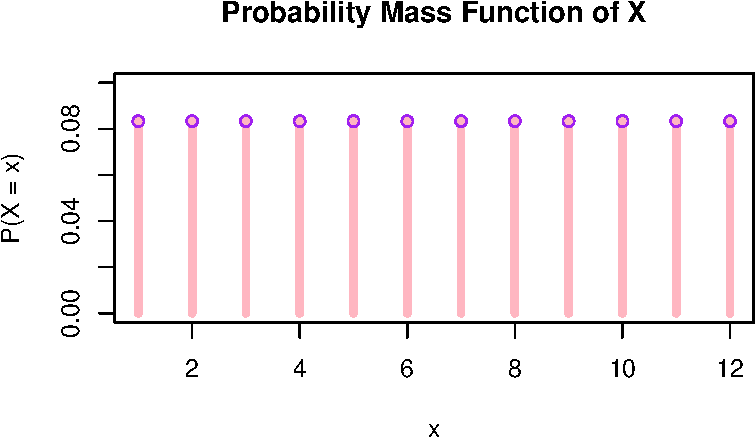
\includegraphics[keepaspectratio]{econ_3201_a1_files/figure-pdf/unnamed-chunk-9-1.pdf}}

\end{tcolorbox}

\begin{enumerate}
\def\labelenumi{(\alph{enumi})}
\setcounter{enumi}{1}
\tightlist
\item
  Plot the cumulative probability distribution function \(f_X(x) in R\).
\end{enumerate}

\begin{tcolorbox}[enhanced jigsaw, arc=.35mm, bottomrule=.15mm, breakable, colback=white, colframe=quarto-callout-tip-color-frame, left=2mm, leftrule=.75mm, opacityback=0, rightrule=.15mm, toprule=.15mm]

\[F_X(x)=P(X\leq x)=
\begin{cases}
0, & x<1,\\
\frac{x}{12}, & 1\leq x<12,\\
1, & x\geq 12.
\end{cases}\]

\begin{Shaded}
\begin{Highlighting}[]
\CommentTok{\# Define the cumulative probabilities}
\NormalTok{x }\OtherTok{\textless{}{-}} \DecValTok{1}\SpecialCharTok{:}\DecValTok{12}
\NormalTok{cdf }\OtherTok{\textless{}{-}} \FunctionTok{cumsum}\NormalTok{(}\FunctionTok{rep}\NormalTok{(}\DecValTok{1}\SpecialCharTok{/}\DecValTok{12}\NormalTok{, }\DecValTok{12}\NormalTok{))}
\CommentTok{\# Plot the CDF}
\FunctionTok{plot}\NormalTok{(x, cdf,}
     \AttributeTok{type =} \StringTok{"s"}\NormalTok{,}
     \AttributeTok{lwd =} \DecValTok{5}\NormalTok{,}
     \AttributeTok{col =} \StringTok{"lightpink"}\NormalTok{,}
     \AttributeTok{main =} \StringTok{"cumulative probability function of X"}\NormalTok{,}
     \AttributeTok{xlab =} \StringTok{"x"}\NormalTok{,}
     \AttributeTok{ylab =} \StringTok{"f(x)"}\NormalTok{,}
     \AttributeTok{ylim =} \FunctionTok{c}\NormalTok{(}\DecValTok{0}\NormalTok{, }\DecValTok{1}\NormalTok{))}

\FunctionTok{points}\NormalTok{(x, cdf, }\AttributeTok{col =} \StringTok{"purple"}\NormalTok{, }\AttributeTok{pch =} \DecValTok{4}\NormalTok{)}
\end{Highlighting}
\end{Shaded}

\pandocbounded{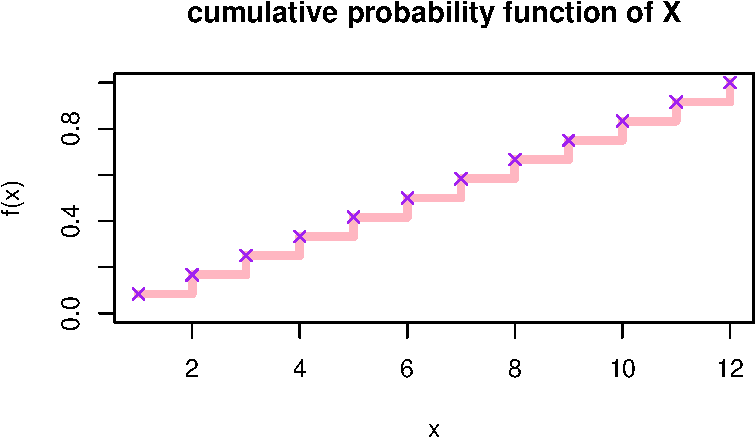
\includegraphics[keepaspectratio]{econ_3201_a1_files/figure-pdf/unnamed-chunk-10-1.pdf}}

```

\end{tcolorbox}

\begin{enumerate}
\def\labelenumi{(\alph{enumi})}
\setcounter{enumi}{2}
\tightlist
\item
  Compute the expected value of \(X\) in R.
\end{enumerate}

\begin{tcolorbox}[enhanced jigsaw, arc=.35mm, bottomrule=.15mm, breakable, colback=white, colframe=quarto-callout-tip-color-frame, left=2mm, leftrule=.75mm, opacityback=0, rightrule=.15mm, toprule=.15mm]

\begin{Shaded}
\begin{Highlighting}[]
\CommentTok{\# Compute expected value: E[X] = sum(x * P(X=x))}
\NormalTok{x }\OtherTok{\textless{}{-}} \DecValTok{1}\SpecialCharTok{:}\DecValTok{12}
\NormalTok{pmf }\OtherTok{\textless{}{-}} \FunctionTok{rep}\NormalTok{(}\DecValTok{1}\SpecialCharTok{/}\DecValTok{12}\NormalTok{, }\DecValTok{12}\NormalTok{)}
\NormalTok{expected\_value }\OtherTok{\textless{}{-}} \FunctionTok{sum}\NormalTok{(x }\SpecialCharTok{*}\NormalTok{ pmf)}
\NormalTok{expected\_value}
\end{Highlighting}
\end{Shaded}

\begin{verbatim}
[1] 6.5
\end{verbatim}

\end{tcolorbox}

\begin{enumerate}
\def\labelenumi{(\alph{enumi})}
\setcounter{enumi}{3}
\tightlist
\item
  Compute the variance of \(X\) in R.
\end{enumerate}

\begin{tcolorbox}[enhanced jigsaw, arc=.35mm, bottomrule=.15mm, breakable, colback=white, colframe=quarto-callout-tip-color-frame, left=2mm, leftrule=.75mm, opacityback=0, rightrule=.15mm, toprule=.15mm]

\begin{Shaded}
\begin{Highlighting}[]
\CommentTok{\# Compute variance: Var(X) = E[X\^{}2] {-} (E[X])\^{}2}
\NormalTok{x }\OtherTok{\textless{}{-}} \DecValTok{1}\SpecialCharTok{:}\DecValTok{12}
\NormalTok{pmf }\OtherTok{\textless{}{-}} \FunctionTok{rep}\NormalTok{(}\DecValTok{1}\SpecialCharTok{/}\DecValTok{12}\NormalTok{, }\DecValTok{12}\NormalTok{)}
\NormalTok{expected\_value }\OtherTok{\textless{}{-}} \FunctionTok{sum}\NormalTok{(x }\SpecialCharTok{*}\NormalTok{ pmf)}

\NormalTok{variance }\OtherTok{\textless{}{-}} \FunctionTok{sum}\NormalTok{((x}\SpecialCharTok{\^{}}\DecValTok{2}\NormalTok{) }\SpecialCharTok{*}\NormalTok{ pmf) }\SpecialCharTok{{-}}\NormalTok{ (expected\_value)}\SpecialCharTok{\^{}}\DecValTok{2}
\NormalTok{variance}
\end{Highlighting}
\end{Shaded}

\begin{verbatim}
[1] 11.91667
\end{verbatim}

\end{tcolorbox}

\subsection{Q6}\label{q6}

The standard normal distribution function is given by
\[f(x)=\frac{e^{-(x^2/2)}}{\sqrt{2\pi}\sigma}\]

\begin{description}
\tightlist
\item[term]
\end{description}

\begin{enumerate}
\def\labelenumi{(\alph{enumi})}
\tightlist
\item
  Define this function in R. (Note: \(\pi\) is coded as \texttt{pi} and
  \(e\) is coded as \texttt{exp}.
\end{enumerate}

\begin{tcolorbox}[enhanced jigsaw, arc=.35mm, bottomrule=.15mm, breakable, colback=white, colframe=quarto-callout-tip-color-frame, left=2mm, leftrule=.75mm, opacityback=0, rightrule=.15mm, toprule=.15mm]

\begin{Shaded}
\begin{Highlighting}[]
\CommentTok{\#Define the standard Normal Distribution}
\NormalTok{f }\OtherTok{\textless{}{-}} \ControlFlowTok{function}\NormalTok{(x)}
  \FunctionTok{exp}\NormalTok{(}\SpecialCharTok{{-}}\NormalTok{(x}\SpecialCharTok{\^{}}\DecValTok{2}\NormalTok{)}\SpecialCharTok{/}\DecValTok{2}\NormalTok{) }\SpecialCharTok{/} \FunctionTok{sqrt}\NormalTok{(}\DecValTok{2}\SpecialCharTok{*}\NormalTok{pi}\SpecialCharTok{*}\DecValTok{1}\NormalTok{)}
\FunctionTok{print}\NormalTok{(f)}
\end{Highlighting}
\end{Shaded}

\begin{verbatim}
function (x) 
exp(-(x^2)/2)/sqrt(2 * pi * 1)
\end{verbatim}

\end{tcolorbox}

\begin{enumerate}
\def\labelenumi{(\alph{enumi})}
\setcounter{enumi}{1}
\tightlist
\item
  Integrate this function over the limit {[}\(-\infty,\infty\){]} using
  the \texttt{integrate()} command in R. Infinity in R is written as
  \texttt{Inf}. To evaluate the integral, use
  \texttt{integrate()\$value}
\end{enumerate}

\begin{tcolorbox}[enhanced jigsaw, arc=.35mm, bottomrule=.15mm, breakable, colback=white, colframe=quarto-callout-tip-color-frame, left=2mm, leftrule=.75mm, opacityback=0, rightrule=.15mm, toprule=.15mm]

\begin{Shaded}
\begin{Highlighting}[]
\NormalTok{integral}\OtherTok{\textless{}{-}}\FunctionTok{integrate}\NormalTok{(f,}\SpecialCharTok{{-}}\ConstantTok{Inf}\NormalTok{,}\ConstantTok{Inf}\NormalTok{)}\SpecialCharTok{$}\NormalTok{value}

\NormalTok{integral}
\end{Highlighting}
\end{Shaded}

\begin{verbatim}
[1] 1
\end{verbatim}

\end{tcolorbox}

\begin{enumerate}
\def\labelenumi{(\alph{enumi})}
\setcounter{enumi}{2}
\tightlist
\item
  Compute the expected value of the standard normal distribution in R
  and confirm it is equal to 0.
\end{enumerate}

\begin{tcolorbox}[enhanced jigsaw, arc=.35mm, bottomrule=.15mm, breakable, colback=white, colframe=quarto-callout-tip-color-frame, left=2mm, leftrule=.75mm, opacityback=0, rightrule=.15mm, toprule=.15mm]

\begin{Shaded}
\begin{Highlighting}[]
\CommentTok{\# Expected value of a f}
\CommentTok{\# Integrate from negative infinity to positive infinity}
\NormalTok{expected\_value\_normal}\OtherTok{\textless{}{-}} \FunctionTok{integrate}\NormalTok{(}\ControlFlowTok{function}\NormalTok{(x) x }\SpecialCharTok{*} \FunctionTok{f}\NormalTok{(x), }\SpecialCharTok{{-}}\ConstantTok{Inf}\NormalTok{, }\ConstantTok{Inf}\NormalTok{)}\SpecialCharTok{$}\NormalTok{value}
\NormalTok{expected\_value\_normal}
\end{Highlighting}
\end{Shaded}

\begin{verbatim}
[1] 0
\end{verbatim}

\end{tcolorbox}

\begin{enumerate}
\def\labelenumi{(\alph{enumi})}
\setcounter{enumi}{3}
\tightlist
\item
  Compute the variance of the standard normal distribution in R and
  confirm it is equal to 1.
\end{enumerate}

\begin{tcolorbox}[enhanced jigsaw, arc=.35mm, bottomrule=.15mm, breakable, colback=white, colframe=quarto-callout-tip-color-frame, left=2mm, leftrule=.75mm, opacityback=0, rightrule=.15mm, toprule=.15mm]

\begin{Shaded}
\begin{Highlighting}[]
\CommentTok{\#Variance of f}
\CommentTok{\# Integrate from negative infinity to positive infinity}
\NormalTok{variance}\OtherTok{\textless{}{-}} \FunctionTok{integrate}\NormalTok{(}\ControlFlowTok{function}\NormalTok{(x) x}\SpecialCharTok{\^{}}\DecValTok{2} \SpecialCharTok{*} \FunctionTok{f}\NormalTok{(x), }\SpecialCharTok{{-}}\ConstantTok{Inf}\NormalTok{, }\ConstantTok{Inf}\NormalTok{)}\SpecialCharTok{$}\NormalTok{value}
\NormalTok{variance}
\end{Highlighting}
\end{Shaded}

\begin{verbatim}
[1] 1
\end{verbatim}

\end{tcolorbox}

\begin{enumerate}
\def\labelenumi{(\alph{enumi})}
\setcounter{enumi}{4}
\tightlist
\item
  Compute \(Pr(Z\leq 0.83)\)
\end{enumerate}

\begin{tcolorbox}[enhanced jigsaw, arc=.35mm, bottomrule=.15mm, breakable, colback=white, colframe=quarto-callout-tip-color-frame, left=2mm, leftrule=.75mm, opacityback=0, rightrule=.15mm, toprule=.15mm]

\begin{Shaded}
\begin{Highlighting}[]
\FunctionTok{integrate}\NormalTok{(f, }\SpecialCharTok{{-}}\ConstantTok{Inf}\NormalTok{, }\FloatTok{0.83}\NormalTok{)}\SpecialCharTok{$}\NormalTok{value}
\end{Highlighting}
\end{Shaded}

\begin{verbatim}
[1] 0.7967306
\end{verbatim}

\end{tcolorbox}

\begin{enumerate}
\def\labelenumi{(\alph{enumi})}
\setcounter{enumi}{5}
\tightlist
\item
  Compute \(Pr(-0.83 \leq Z\leq 0.83)\)
\end{enumerate}

\begin{tcolorbox}[enhanced jigsaw, arc=.35mm, bottomrule=.15mm, breakable, colback=white, colframe=quarto-callout-tip-color-frame, left=2mm, leftrule=.75mm, opacityback=0, rightrule=.15mm, toprule=.15mm]

\begin{Shaded}
\begin{Highlighting}[]
\FunctionTok{integrate}\NormalTok{(f, }\SpecialCharTok{{-}}\FloatTok{0.83}\NormalTok{, }\FloatTok{0.83}\NormalTok{)}\SpecialCharTok{$}\NormalTok{value}
\end{Highlighting}
\end{Shaded}

\begin{verbatim}
[1] 0.5934612
\end{verbatim}

\end{tcolorbox}

\begin{enumerate}
\def\labelenumi{(\alph{enumi})}
\setcounter{enumi}{6}
\tightlist
\item
  Compute \(Pr(-0.83 \leq Z\leq 0.83)\) using the \texttt{pnorm()}
  command and compare your results to (f).
\end{enumerate}

\begin{tcolorbox}[enhanced jigsaw, arc=.35mm, bottomrule=.15mm, breakable, colback=white, colframe=quarto-callout-tip-color-frame, left=2mm, leftrule=.75mm, opacityback=0, rightrule=.15mm, toprule=.15mm]

\begin{Shaded}
\begin{Highlighting}[]
\FunctionTok{pnorm}\NormalTok{(}\FloatTok{0.83}\NormalTok{)}\SpecialCharTok{{-}} \FunctionTok{pnorm}\NormalTok{(}\SpecialCharTok{{-}}\FloatTok{0.83}\NormalTok{)}
\end{Highlighting}
\end{Shaded}

\begin{verbatim}
[1] 0.5934612
\end{verbatim}

\end{tcolorbox}

\subsection{Q7}\label{q7}

Let \(X\) denote the prison sentence, in years, for people convicted of
auto theft in a particular province in Canada. Suppose the PDF of \(X\)
is given by: \[f(X)=\frac{1}{9}x^2,\text{ }0<x<3.\]

\begin{enumerate}
\def\labelenumi{(\alph{enumi})}
\tightlist
\item
  Define \(f(x)\) in R.
\end{enumerate}

\begin{tcolorbox}[enhanced jigsaw, arc=.35mm, bottomrule=.15mm, breakable, colback=white, colframe=quarto-callout-tip-color-frame, left=2mm, leftrule=.75mm, opacityback=0, rightrule=.15mm, toprule=.15mm]

\begin{Shaded}
\begin{Highlighting}[]
\CommentTok{\#Define the PDF}
\CommentTok{\#Define the standard Normal Distribution}
\NormalTok{f }\OtherTok{\textless{}{-}}\NormalTok{ (}\FunctionTok{f}\NormalTok{ (x))}
\NormalTok{f }\OtherTok{\textless{}{-}} \ControlFlowTok{function}\NormalTok{(x)}
\NormalTok{  x}\SpecialCharTok{\^{}}\DecValTok{2}\SpecialCharTok{/}\DecValTok{9}
\FunctionTok{print}\NormalTok{(f)}
\end{Highlighting}
\end{Shaded}

\begin{verbatim}
function (x) 
x^2/9
\end{verbatim}

\end{tcolorbox}

\begin{enumerate}
\def\labelenumi{(\alph{enumi})}
\setcounter{enumi}{1}
\tightlist
\item
  Integrate \(f(x)\) over the interval {[}0,3{]}.
\end{enumerate}

\begin{tcolorbox}[enhanced jigsaw, arc=.35mm, bottomrule=.15mm, breakable, colback=white, colframe=quarto-callout-tip-color-frame, left=2mm, leftrule=.75mm, opacityback=0, rightrule=.15mm, toprule=.15mm]

\begin{Shaded}
\begin{Highlighting}[]
\NormalTok{integral}\OtherTok{\textless{}{-}}\FunctionTok{integrate}\NormalTok{(f,}\DecValTok{0}\NormalTok{,}\DecValTok{3}\NormalTok{)}\SpecialCharTok{$}\NormalTok{value}

\NormalTok{integral}
\end{Highlighting}
\end{Shaded}

\begin{verbatim}
[1] 1
\end{verbatim}

\end{tcolorbox}

\begin{enumerate}
\def\labelenumi{(\alph{enumi})}
\setcounter{enumi}{2}
\tightlist
\item
  Compute the expected prison sentence.
\end{enumerate}

\begin{tcolorbox}[enhanced jigsaw, arc=.35mm, bottomrule=.15mm, breakable, colback=white, colframe=quarto-callout-tip-color-frame, left=2mm, leftrule=.75mm, opacityback=0, rightrule=.15mm, toprule=.15mm]

\begin{Shaded}
\begin{Highlighting}[]
\CommentTok{\# Expected value of a f}
\CommentTok{\# Integrate from 0 to 3}
\NormalTok{expected\_value\_normal}\OtherTok{\textless{}{-}} \FunctionTok{integrate}\NormalTok{(}\ControlFlowTok{function}\NormalTok{(x) x}\SpecialCharTok{*}\NormalTok{  x}\SpecialCharTok{\^{}}\DecValTok{2}\SpecialCharTok{/}\DecValTok{9}\NormalTok{, }\DecValTok{0}\NormalTok{, }\DecValTok{3}\NormalTok{)}\SpecialCharTok{$}\NormalTok{value}
\NormalTok{expected\_value\_normal}
\end{Highlighting}
\end{Shaded}

\begin{verbatim}
[1] 2.25
\end{verbatim}

\end{tcolorbox}

\subsection{Q8}\label{q8}

Let \(X\) follow a Student \(t\) distribution with \(M\) degrees of
freedom. Then \[X=\frac{Z}{\sqrt{W/M}}\sim t_M,\] where \(Z\) is a
standard normal variable and \(W\) is a chi-squared variable with \(M\)
degrees of freedom.

\begin{enumerate}
\def\labelenumi{(\alph{enumi})}
\tightlist
\item
  On the same figure plot the following:

  \begin{enumerate}
  \def\labelenumii{(\roman{enumii})}
  \tightlist
  \item
    Plot the standard normal probability distribution using
    \texttt{curve()}. Specify the range as {[}-5,5{]} using
    \texttt{xlim}. Name the \texttt{ylab} ``Density''. The main title
    should be ``Densities of t Distribution''.
  \item
    Plot the Student t distribution with 5 degrees of freedom using
    \texttt{curve()} and \texttt{dt()}. Specify the range as {[}-5,5{]}
    using \texttt{xlim}. Choose a different colour, i.e.~\texttt{col=2}.
    To learn more about \texttt{dt}, type \texttt{?dt} in your console.
  \item
    Plot the Student t distribution with 15 degrees of freedom using
    \texttt{curve()} and \texttt{dt()}. Specify the range as {[}-5,5{]}
    using \texttt{xlim}. Choose a different colour, i.e.~\texttt{col=3}.
    To learn more about \texttt{dt}, type \texttt{?dt} in your console.
  \item
    Plot the Student t distribution with 25 degrees of freedom using
    \texttt{curve()} and \texttt{dt()}. Specify the range as {[}-5,5{]}
    using \texttt{xlim}. Choose a different colour, i.e.~\texttt{col=4}.
    To learn more about \texttt{dt}, type \texttt{?dt} in your console.
  \item
    Include the following legend in you plot:\\
    \texttt{legend("topright",}~
    \texttt{c("N(0,\ 1)",\ "M=2",\ "M=4",\ "M=25"),}~
    \texttt{col\ =\ 1:4,}~ \texttt{lty\ =\ c(1,\ 1,\ 1,\ 1))}\\
  \end{enumerate}
\end{enumerate}

\begin{tcolorbox}[enhanced jigsaw, arc=.35mm, bottomrule=.15mm, breakable, colback=white, colframe=quarto-callout-tip-color-frame, left=2mm, leftrule=.75mm, opacityback=0, rightrule=.15mm, toprule=.15mm]

\begin{Shaded}
\begin{Highlighting}[]
\CommentTok{\# (a) Plot the standard normal and Student t distributions}

\CommentTok{\# (i) Standard Normal Distribution}
\FunctionTok{curve}\NormalTok{(}\FunctionTok{dnorm}\NormalTok{(x), }\AttributeTok{from =} \SpecialCharTok{{-}}\DecValTok{5}\NormalTok{, }\AttributeTok{to =} \DecValTok{5}\NormalTok{,}
\AttributeTok{xlab =} \FunctionTok{c}\NormalTok{(}\SpecialCharTok{{-}}\DecValTok{5}\NormalTok{,}\DecValTok{5}\NormalTok{), }\AttributeTok{ylab =} \StringTok{"Density"}\NormalTok{,}
\AttributeTok{main =} \StringTok{"Densities of t Distribution"}\NormalTok{,}
\AttributeTok{col =} \StringTok{"1"}\NormalTok{)}

\CommentTok{\# (ii) Student T distribution, df=5}
\FunctionTok{curve}\NormalTok{(}\FunctionTok{dt}\NormalTok{(x, }\AttributeTok{df =}\DecValTok{5}\NormalTok{),}
            \AttributeTok{from =} \DecValTok{5}\NormalTok{, }\AttributeTok{to =} \SpecialCharTok{{-}}\DecValTok{5}\NormalTok{,}
            \AttributeTok{xlab =} \FunctionTok{c}\NormalTok{(}\SpecialCharTok{{-}}\DecValTok{5}\NormalTok{,}\DecValTok{5}\NormalTok{), }\AttributeTok{ylab =} \StringTok{"Density"}\NormalTok{,}
            \AttributeTok{col =} \StringTok{"2"}\NormalTok{,}\AttributeTok{add =} \ConstantTok{TRUE}\NormalTok{)}
\NormalTok{?dt}

\CommentTok{\# (iii) Student T distribution df=15}
\FunctionTok{curve}\NormalTok{(}\FunctionTok{dt}\NormalTok{(x, }\AttributeTok{df =} \DecValTok{15}\NormalTok{),}
            \AttributeTok{from =} \DecValTok{5}\NormalTok{, }\AttributeTok{to =} \SpecialCharTok{{-}}\DecValTok{5}\NormalTok{,}
            \AttributeTok{xlab =} \FunctionTok{c}\NormalTok{(}\SpecialCharTok{{-}}\DecValTok{5}\NormalTok{,}\DecValTok{5}\NormalTok{), }\AttributeTok{ylab =} \StringTok{"Density"}\NormalTok{,}
            \AttributeTok{col =} \StringTok{"3"}\NormalTok{, }\AttributeTok{add =} \ConstantTok{TRUE}\NormalTok{)}
\NormalTok{?dt}

\CommentTok{\#(iv) Student T distribution df=25}
\FunctionTok{curve}\NormalTok{(}\FunctionTok{dt}\NormalTok{(x, }\AttributeTok{df =}\DecValTok{25}\NormalTok{),}
            \AttributeTok{from =} \DecValTok{5}\NormalTok{, }\AttributeTok{to =} \SpecialCharTok{{-}}\DecValTok{5}\NormalTok{,}
            \AttributeTok{xlab =} \FunctionTok{c}\NormalTok{(}\SpecialCharTok{{-}}\DecValTok{5}\NormalTok{,}\DecValTok{5}\NormalTok{), }\AttributeTok{ylab =} \StringTok{"Density"}\NormalTok{,}
            \AttributeTok{col =} \StringTok{"4"}\NormalTok{,}\AttributeTok{add =} \ConstantTok{TRUE}\NormalTok{)}
\NormalTok{?dt}
\CommentTok{\#(v) }
\FunctionTok{legend}\NormalTok{(}\StringTok{"topright"}\NormalTok{,}
       \FunctionTok{c}\NormalTok{(}\StringTok{"N(0, 1)"}\NormalTok{, }\StringTok{"M=5"}\NormalTok{, }\StringTok{"M=15"}\NormalTok{, }\StringTok{"M=25"}\NormalTok{),}
       \AttributeTok{col =} \DecValTok{1}\SpecialCharTok{:}\DecValTok{4}\NormalTok{,}
       \AttributeTok{lty =} \FunctionTok{c}\NormalTok{(}\DecValTok{1}\NormalTok{, }\DecValTok{1}\NormalTok{, }\DecValTok{1}\NormalTok{, }\DecValTok{1}\NormalTok{))}
\end{Highlighting}
\end{Shaded}

\pandocbounded{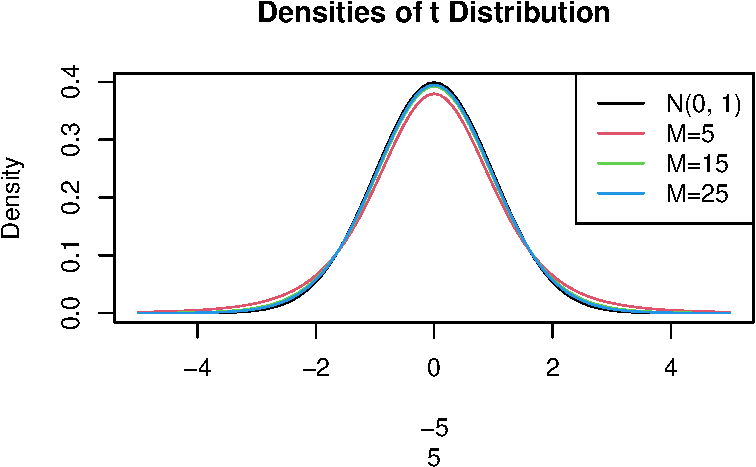
\includegraphics[keepaspectratio]{econ_3201_a1_files/figure-pdf/unnamed-chunk-23-1.pdf}}

\end{tcolorbox}

\begin{enumerate}
\def\labelenumi{(\alph{enumi})}
\setcounter{enumi}{1}
\tightlist
\item
  What do you observe as the degrees of freedom increase?
\end{enumerate}

\begin{tcolorbox}[enhanced jigsaw, arc=.35mm, bottomrule=.15mm, breakable, colback=white, colframe=quarto-callout-tip-color-frame, left=2mm, leftrule=.75mm, opacityback=0, rightrule=.15mm, toprule=.15mm]

As the degrees of freedom increase, the Student t distribution
approaches the standard normal distribution. It also confirms the
central limit theorm, that is as n becomes larger, the actual function
becomes better appoximated by the normal distribution

\end{tcolorbox}

\#quarto render econ\_3201\_a1.qmd --to pdf




\end{document}
